\section{Метод}

\subsection{Многоканальные vertex‐to‐ROI функциональные коннектомы}

Входными данными для моделей прогнозирования являются функциональные коннектомы, представленные в виде многоканальных данных, прикрепленных к вершинам икосаэдрической сетки.
На рис.\ref{BrSurf2} показана конструкция многоканальных функциональных коннектомов vertex-to-ROI (из вершины в интересующий регион), используемых в наших экспериментах.
Такая функциональная связь задается формулой:

\begin{figure}
\centering
\includegraphics[scale=0.4]{fig/fig1.png}
\caption{\footnotesize{Многоканальные функциональные коннектомы vertex-to-ROI, вычисленные на основе rsfMRI}}
\label{BrSurf2}
\end{figure}

\begin{equation}
    \boldsymbol{r}_{ij} = corr(\boldsymbol{t}_i, \bar{\boldsymbol{t}}_j)
\end{equation}

где $\boldsymbol{r}_{ij}$ представляет собой функциональную связность между $i$-ой вершиной поверхности и $j$-ым интересующим регионом, и вычисляется как коэффициент корреляции Пирсона $corr(.)$  между временными рядами $\textbf{t}_i$ rsfMRI в $i$-й вершине и средним значением временных рядов $\bar{\textbf{t}}_j$ для $j$-го интересующего региона.
В наших экспериментах шаблоном поверхности является fs$\_$LR шаблон с $32 492$ вершинами (\cite{van2012parcellations}).
ROI -- это парсели (регионы), полученные на основе группового независимого компонентного анализа (ICA) (\cite{smith2013resting}), в котором $50$ компонентов были рассчитаны на основе временных рядов fMRI в состоянии покоя объектов обучения (поэтому испытуемые были исключены из ICA).
Каждой вершине присваивается метка участка, соответствующая компоненту с наибольшим значением z-балла в данном местоположении.
Из всех значений ROI $42$ лежат на кортикальной поверхности.
Коннектомы каждого объекта из двух полушарий могут быть объединены, в результате чего получается единая входная икосаэдрическая сетка с количеством каналов, в два раза превышающим количество ROI.
Следовательно, результирующий функциональный коннектом каждого субъекта представляет собой сетку из $32,492$ вершин с $84$ каналами.

Использование корреляции временных рядов rsfMRI между вершинами и ROI для определения функциональной связности мозга является широко распространенной практикой в нейровизуализационном анализе.
По сравнению с функциональными коннектомами ROI-to-ROI и плотными функциональными коннектомами vertex-to-vertex, функциональные коннектомы vertex-to-ROI обеспечивают баланс между представлением с высоким пространственным разрешением, необходимым для моделей прогнозирования, и при этом остаются выполнимыми с точки зрения вычислений.


\subsection{Модель BrainSurfCNN}

\begin{figure}
\centering
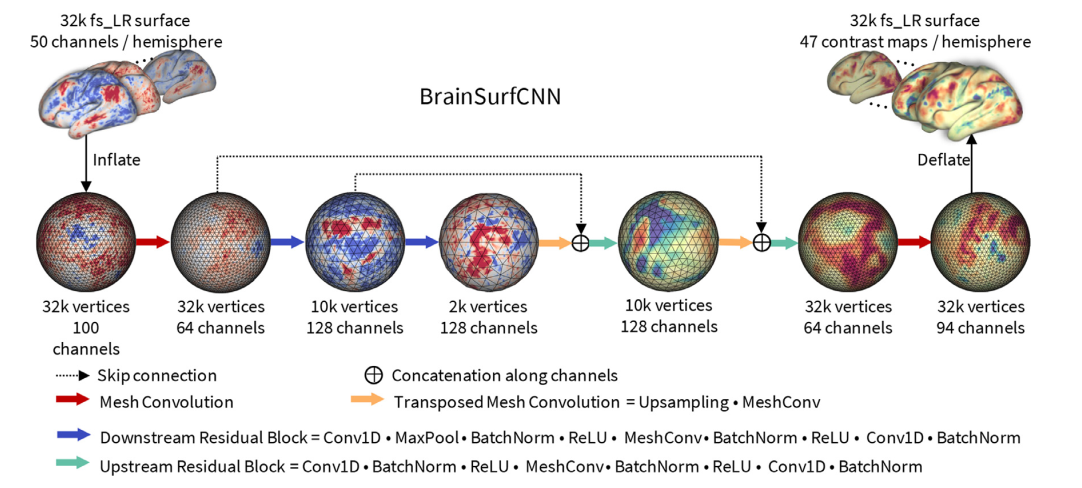
\includegraphics[scale=0.5]{fig/BrainSurfCNN.png}
\caption{\footnotesize {Модель BrainSurfCNN}}
\label{BrSurf}
\end{figure}

На рис.\ref{BrSurf} показана рассматриваемая модель BrainSurfCNN для прогнозирования различий между задачами и функциональными коннектомами в состоянии покоя.
BrainSurfCNN основана на архитектуре UNet (\cite{ronneberger2015u}) и использует сферическое сверточное ядро для работы со сферической сеткой.
Наиболее заметной особенностью архитектуры UNet являются пропускные соединения, которые копируют функции из блока кодирования (выходы из нижних блоках на рис.\ref{BrSurf}) на входы блока декодирования (входы для верхних блоках на рис.\ref{BrSurf}).
Входная и выходная поверхности представляют собой шаблоны fs$\_$LR с $32,492$ вершинами (поверхность fs$\_$LR $32$k) на каждое полушарие мозга.
Левое и правое полушария симметричны в атласах fs$\_$LR, т.е. одинаковый индекс вершины в обоих полушариях соответствует противоположным гомологам.
Таким образом, коннектомы каждого объекта из двух полушарий могут быть объединены, в результате чего получается единая входная икосаэдрическая сетка с количеством каналов, в два раза превышающим количество ROI.
На выходе BrainSurfCNN также представляет собой многоканальную икосаэдрическую сетку, в которой каждый канал соответствует контрасту для одной задачи МРТ.
% Эта настройка многозадачного прогнозирования способствует распределению веса между прогнозируемыми контрастами.


\subsection{Функция потерь}

В процессе обучения модели BrainSurfCNN минимизируется реконструктивно-контрастивная функция потерь (RC loss, \cite{koch2015siamese}). 
RC loss связан с метрическим обучением, и также применим к задаче генерации изображений в области нейронауки.

Дан минибатч из $N$ сэмплов: $B=\{\textbf{x}_i\}$., в котором
$\textbf{x}_i$ представляет собой  целевое многоконтрастное изображение объекта $i$, пусть $\hat{\textbf{x}}_i$ определяет соответствующее прогнозируемое изображение контраста. Тогда RC loss можно выразить как:
\begin{equation}
    \mathcal{L}_R = \frac{1}{N} \sum\limits_{i=1}^N d(\hat{\textbf{x}}_i, {\textbf{x}}_i),
\end{equation} 

\begin{equation}
    \mathcal{L}_C = \frac{1}{(N^2-N)/2} \sum\limits_{\substack{\textbf{x}_j \in B_i, \\ j\neq i}} d(\hat{\textbf{x}}_i, {\textbf{x}}_j),
\end{equation}

\begin{equation}
    \mathcal{L}_{RC} = [\mathcal{L}_R - \alpha]_+ + [\mathcal{L}_R - \mathcal{L}_C + \beta]_+,
\end{equation}
где $d(.)$ является функцией потерь (например, $l_2$-нормой, которая и была использована в экспериментах).
$\mathcal{L}_R, \alpha$ -- потери и отступ (margin) для одного и то же объекта (R loss).
$\mathcal{L}_C, \beta$ -- потери и отступ (margin) для разных объектов (C loss). 
В совокупности получаем $\mathcal {L}_{RC}$, что приводит к тому, что ошибка по одному и тому же объекту $\mathcal{L}_{R}$ находится в пределах допустимого значения $\alpha$, в то время как разница по разным объектам $\mathcal{L}_{C}$ является такой большой, что $(\mathcal{L}_C-\mathcal{L}_R) > \beta$.
% Как были установлены $\alpha$ и $\beta$ на практике, описано ниже.


\subsection{Основная модель (baseline)}
\subsubsection{Линейная регрессия}

Основная модель линейной регрессии (\cite{tavor2016task}) представлена как:
\begin{equation}
    \boldsymbol{y}_i^k = \boldsymbol{X}_i^k \boldsymbol{\beta}_i^k,   
\end{equation}
где $\boldsymbol{y}_i^k, \boldsymbol{X}_i^k,  \boldsymbol{\beta}_i^k$ являются патерном активации, входными признаками и регрессором для $k$-го участка в $i$-м объекте, соответственно.
Для вычисления модели линейной регрессии была использована парцелляция из $50$ компонентов, полученная из ICA и предоставленная HCP. 

$\boldsymbol{y}_i^k$ является вектором длины $n_k$, где $n_k$ -- количество вертексов в $k$-ом парселе в обоих полушариях мозга.
$\boldsymbol{X}_i^k$ является функциональной матрицей связности размером  $n_k \times M$, где каждый элемент был вычислен как корреляция Пирсона между вертексом и средним временных рядов каждого из $M$ интересующих регионов (те же временные ряды были использованы для вычисления входных данных модели BrainSurfCNN).
 
Линейная модель была подобрана для каждого участка и каждого контраста задач каждого объекта обучения.
Таким образом, после обучения заданному контрасту задач для каждого участка существует отдельная линейная модель, подобранная для каждого объекта обучения.
Для вычисления прогнозов по данным полученные веса линейных моделей были усреднены по всем объектам, чтобы получить единую прогностическую модель для каждого парселя.
% Отметим, что это соответствует сборке линейных моделей по всем испытуемым.

Предсказанный патерн активации $\hat{\boldsymbol{y}}_{\text{test}}^k$ $k$-го парселя невидимого (не участвовавшего в обучении) объекта исследования вычисляется как:
\begin{equation}
\hat{\boldsymbol{y}}_{\text{test}}^k = {\boldsymbol{X}}_{\text{test}}^k \bar{\boldsymbol{\beta}}^k = {\boldsymbol{X}}_{\text{test}}^k \frac{1}{N_{\text{train}}} \sum_{i=1}^{N_{\text{train}}} {\boldsymbol{\beta}}_i^k = \frac{1}{N_{\text{train}}} \sum_{i=1}^{N_{\text{train}}} {\boldsymbol{X}}_{\text{test}}^k {\boldsymbol{\beta}}_i^k,
\end{equation} 
где $\bar{\boldsymbol{\beta}}^k$ представляет собой усреднённые веса моделей линейной регрессии для $k$-го парселя, вычисленного по $N_\text{train}$ объектам обучения.


\subsubsection{Усреднённые по группе контрасты}
Разная степень вариабельность между индивидами проявляется в различных контрастах задач.
Такая вариабельность была интересна для этого исследования.
Поэтому были использованы средние значения по группе в качестве наивного ориентира.
Усреднённые по группе контрасты также отражают наиболее характерные особенности карты активации, зависимые от условий задачи, что должна учитывать модель прогнозирования.


\subsubsection{Повторяющиеся контрасты}
В этой работе были использованы повторные fMRI-сканирования (при их наличии) для количественной оценки надежности целевых карт контрастов и оценки характеристик прогнозирования модели BrainSurfCNN и новной модели.
Повторные контрасты сравнивались с первоначальными контрастами как с точки зрения общего соответствия (измеренного с помощью игральных костей), так и в задаче идентификации объекта.


\subsection{Метрика качества}
Показатель Dice (\cite{dice1945measures}) используется для измерения степени совпадения между прогнозируемым контрастом и целевой картой контрастности для заданного процента наиболее активированных вершин.
При заданном пороговом значении $x\%$, показатель Dice вычисляется как:
\begin{equation}
    Dice(x) = \frac{2 | Prediction(x) \cap Target(x)|}{| Prediction(x) | + | Target(x)|},
\end{equation}
где $| Prediction(x) |$ определяет  количество топ-$x\%$ наиболее активированных вершин на прогнозируемой карте контрастности, $| Target(x)|$ $| Target(x)|$ определяет количество топ-$x\%$ наиболее активированных вершин в контрасте, и $| Prediction(x) \cap Target(x)|$ определяет количество вершин, которые перекрывают прогнозируемую и целевую карты при заданном пороговом значении. 

При более низком пороговом значении (например, при $5\%$ наиболее активированных вершин) показатель Dice измеряет соответствие мелких деталей между целевым и прогнозируемым контрастами.
При более высоких пороговых значениях (например, $50\%$ наиболее активированных вершин) этот показатель количественно определяет глобальное соответствие анатомических распределений.
Интегрируя показатели Dice по ряду пороговых значений (от $5\%$ до $50\%$ от наиболее активированных вершин с интервалом в $5\%$), мы получаем итоговый показатель - площадь под кривой Dice (Dice AUC) -
для оценки качества предсказания модели.

